\section{System description}
\label{sec:sys}

This section will present a detailed description of our \ac{LTR} system. 
Our system was designed to work by using 3D lidar scans as a primary mean of localization, also using \ac{IMU} and wheel odometry as input. 
The main components of the framework are shown in~\autoref{fig:ltr_flow}.
Incoming lidar scans are registered to a reference map using the \ac{ICP} algorithm in order to localize the robot and build a map of the environment, so the implementation of localization will be described first.
Next, the path following algorithm, consisting of a simple controller and localizing-only \ac{ICP}.
%% Describe map, odom, robot and lidar frames

\begin{figure} [htpb]
	\centering
	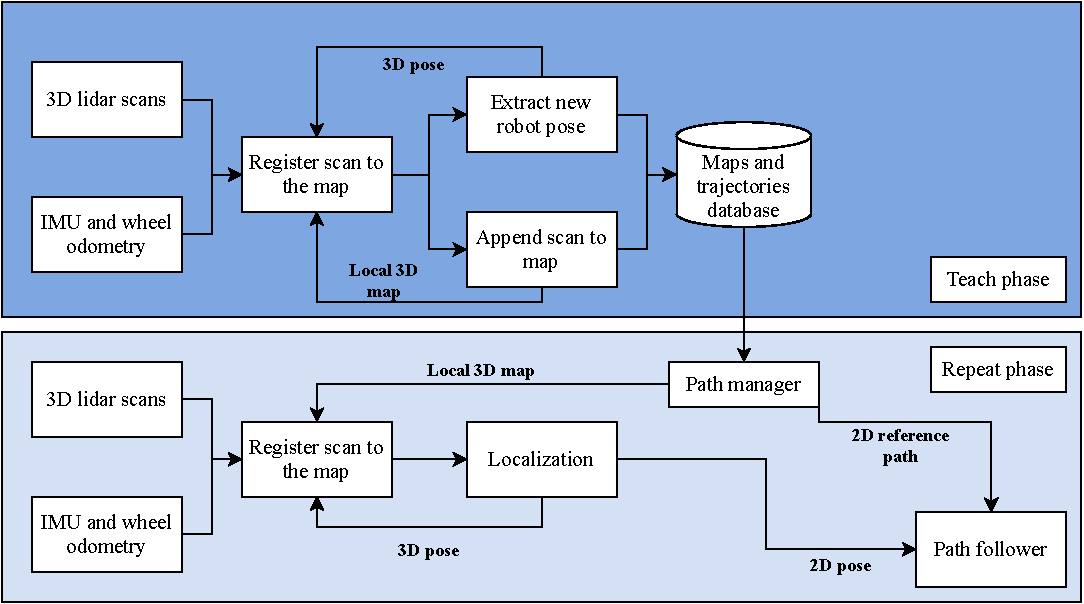
\includegraphics[height=3.2in]{figs/LTR_flowchart.pdf}
	\caption{Flowchart for LTR}
	\label{fig:ltr_flow}
\end{figure}

\begin{figure} [htpb]
	\centering
	\includegraphics[height=2.0in]{example-image}
	\caption{Coordinate frames used for \ac{LTR}}
	\label{fig:ltr_frames}
\end{figure}


\subsection{Lidar teach-and-repeat}
\label{sec:LTR}

Our \ac{LTR} framework was designed to allow to repeat previously driven paths over large distances. 
Localization is done mainly using lidar scans registration through the \ac{ICP} algorithm.
During the teach phase, every \ac{ICP} pose is logged in order to record the path that was driven by the operator.
All registered scans are also logged into a map, with a limit of density of points. 
During the repeat phase, the corresponding map and trajectory are loaded and the robot follows the reference path using a simple controller.
Registered scans are not added to the map during the repeat phase, we have found empirically that not updating the map during repeat runs increases the localization robustness.



\subsubsection{Iterative closest point}
\label{ICP}

\lightlipsum[1]

\begin{figure} [htpb]
	\centering
	\includegraphics[height=2.0in]{example-image}
	\caption{Figure explaining Simon-Pierre's tiled mapping framework}
	\label{fig:tiled_map}
\end{figure}

\begin{table}[htpb]
	\caption{\ac{ICP} parameters} \label{tab:LTR-runs}
	\begin{center}
		\begin{tabular}{|c|c|c|c|c|c|}
			\hline
			% after \\: \hline or \cline{col1-col2} \cline{col3-col4} ...
			& $k_{g}$ & $k_{o}$ & $c_{3}$ & $c_{4}$ & $c_{5}$ \\
			\hline\hline
			Careful/Sparse & 0.334 & 0.597 & 1.101 & 9.621 & 8.170 \\ \hline
			Careful/Dense & 3.124 & 3.195 & 1.094 & 5.899 & 7.318 \\ \hline
			Aggressive/Sparse & 0.840 & 9.153 & 2.853 & 8.274 & 0.187 \\ \hline
			Aggressive/Dense & 4.838 & 2.841 & 0.670 & 7.952 & 0.386 \\ \hline
			Hand-Tuned & 0.767 & 0.060 & 0.340 & 2.000 & 0.250 \\
			\hline
		\end{tabular}
	\end{center}
\end{table}

\subsubsection{Path following}
\label{sec:orthexp}

\lightlipsum[1]

\begin{figure} [htpb]
	\centering
	\includegraphics[height=2.0in]{example-image}
	\caption{Figure explaining Differential orthogonal-exponential controller}
	\label{fig:diff_orthexp}
\end{figure}

\subsection{Hardware description}
\label{sec:hardware}

Our system was deployed on a Clearpath Robotics Warthog \ac{UGV}. 
The Warthog is a \ac{SSMR} using two drive units located on each side of it's chassis. 
The drive
For \acp{SSMR}, steering is done by sending rotating the wheels on each side of the vehicle at different velocities to creating a skidding effect, effectively turning the vehicle.
The Warthog can be equipped with wheels or tracks, for this work, we selected the latter in order to maximize mobility. 
The Warthog is also equipped with a differential suspension, maximizing track or wheel traction when navigating steep terrain.
The warthog is also equipped with a standard sensor suite for autonomous navigation. 
In order to enable the \ac{LTR} framework, a Robosense RS-32 3D lidar is mounted in front of the robot, for this work, it is the only lidar used for localization.
3 Hall effect sensors are added to each motor to provide wheel odometry for the robot. 
Finally, an XSens MTi-10 \ac{IMU} provides angular velocity, body linear acceleration and gravitational acceleration measurements. 
Additional sensors used for recording in this work include a Dalsa C1920 camera and two Emlid Reach-RS+ \ac{GPS} receivers.
Two Robosense RS-16 lidars were added to the rear of the platform to collect measurements on tree canopy but no data was recorded through those sensors. 
All technical specifications for the platform are given in~\autoref{tab:warthog_specs}.

\begin{table}[htpb]
	\caption{Warthog specifications} \label{tab:warthog_specs}
	\begin{center}
		\begin{tabular}{c c c c}
			\textbf{Physical} &  & \textbf{Power} & \\
			% after \\: \hline or \cline{col1-col2} \cline{col3-col4} ...
			Mass & \SI{590}{kg} & Chemistry & AGM sealed lead acid \\ 
			Footprint & 2.13 x 1.52 m & Voltage & \SI{48}{V} \\ 
			Top speed & \SI{18}{km/h} & Capacity & \SI{105}{Ah} \\ 
			Steering geometry & Skid-steering  & Drive & Sevcon Gen4 \\
			Locomotion & CAMSO ATV T4S Tracks \\
			Suspension & Geometric Passive Articulation \\
			\textbf{Sensors} & & \textbf{Computing} \\
			\ac{LTR} & & Computer & Acrosser AIV-Q170V1FL  \\
			Front lidar & Robosense RS-32 (\SI{10}{Hz}) & CPU & i7-6700 TE \\
			\ac{IMU} & XSens MTi-10 (\SI{100}{Hz}) \\ 
			Wheel encoders & 3 x hall effect sensors (\SI{4}{Hz}) \\
			Recording & &   \\
			Camera & Dalsa C1920 (\SI{8}{Hz})  \\
			\ac{GPS} & Emlid Reach-RS+ (\SI{5}{Hz}) \\
		\end{tabular}
	\end{center}
\end{table}

\begin{figure} [htpb]
	\centering
	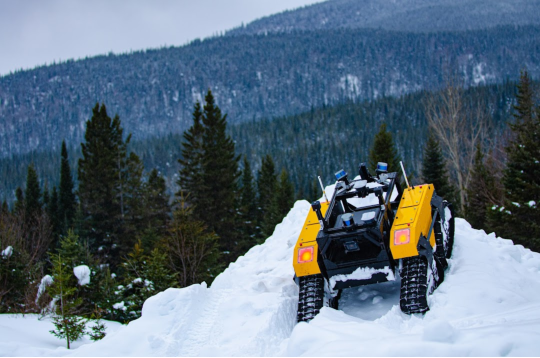
\includegraphics[height=4.0in]{figs/warthog_sys_description.pdf}
	\caption{Warthog figure, pointing to every sensor.}
	\label{fig:warthog}
\end{figure}
%% To do : Edit Figure to add pointers for all sensors